\documentclass[tikz, border=5mm]{standalone}

\usepackage{amsmath, amssymb, standalone}
\usetikzlibrary{arrows.meta, positioning}
\usetikzlibrary{decorations.pathreplacing}
\tikzstyle{box} = [rectangle, rounded corners, 
minimum width=3cm, 
minimum height=1cm,
align=center, 
draw=black, 
fill=blue!30]
\tikzstyle{arrow} = [->,thick]


\begin{document}
		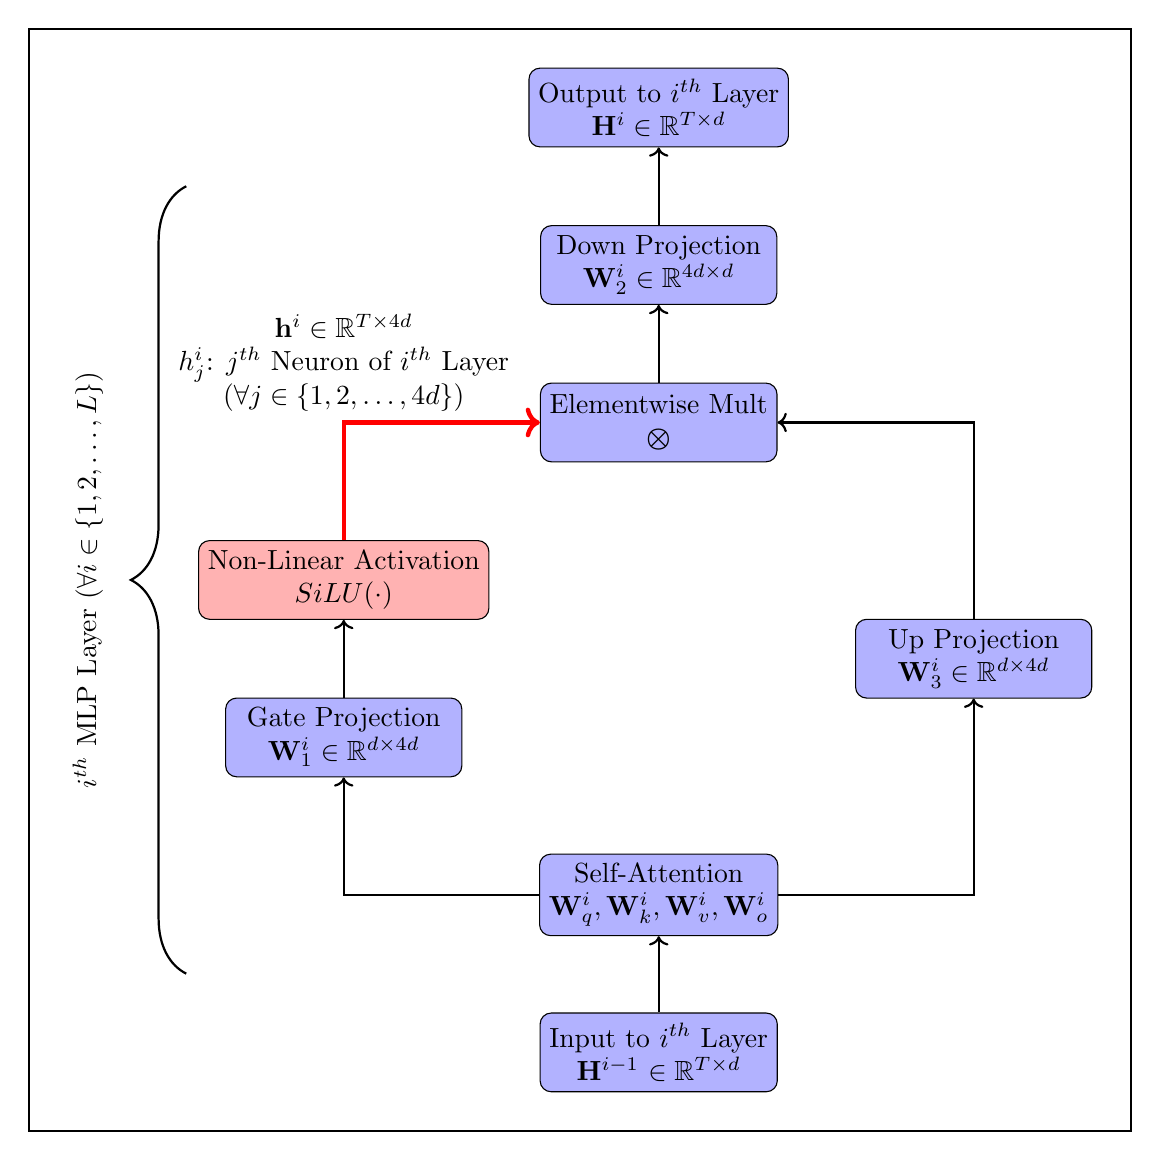
\begin{tikzpicture}
				
				% Define the canvas boundary (optional, for visualization)
				\draw[thick, black] (0,0) rectangle (14,14);
%				\draw[step=1cm,gray,very thin] (0,0) grid (16,16);
				
				\node[box] (input) at (8,1) {Input to $i^{th}$ Layer \\ $\mathbf{H}^{i-1}$  $\in \mathbb{R}^{T \times d}$};
				\node[box] (selfattn) at ([xshift=0cm, yshift=2cm]input.center) {Self-Attention \\ $\mathbf{W}_q^i, \mathbf{W}_k^i, \mathbf{W}_v^i, \mathbf{W}_o^i$};
				\node[box] (W1) at ([xshift=-4cm, yshift=2cm]selfattn.center) {Gate Projection \\ $\mathbf{W}_1^i \in \mathbb{R}^{d \times 4d}$};
				\node[box] (W3) at ([xshift=4cm, yshift=3cm]selfattn.center) {Up Projection \\ $\mathbf{W}_3^i \in \mathbb{R}^{d \times 4d}$};
				\node[box, fill=red!30] (silu) at ([xshift=0cm, yshift=2cm]W1.center) {Non-Linear Activation \\ $SiLU(\cdot)$};
				\node[box] (mult) at ([xshift=4cm, yshift=2cm]silu.center) {Elementwise Mult \\ $\boldsymbol{\otimes}$} ;
				\node[box] (W2) at ([xshift=0cm, yshift=2cm]mult.center) {Down Projection \\ $\mathbf{W}_2^i \in \mathbb{R}^{4d \times d}$};
				\node[box] (output) at ([xshift=0cm, yshift=2cm]W2.center) {Output to $i^{th}$ Layer \\ $\mathbf{H}^{i} \in \mathbb{R}^{T \times d}$};
							
				% Edges
				\draw[arrow] (input) -- (selfattn);
				\draw[arrow] (selfattn) -| (W1);
				\draw[arrow] (selfattn) -| (W3);
				\draw[arrow] (W1) -- (silu);
				\draw[arrow, red, ultra thick] (silu) |- node[anchor=south, align=center, black] {$\mathbf{h}^i \in \mathbb{R}^{T \times 4d}$ \\ $h^i_j$: $j^{th}$ Neuron of $i^{th}$ Layer \\ ($\forall j \in \{1, 2, \dots, 4d\}$)} (mult);
				\draw[arrow] (W3) |- (mult);
				\draw[arrow] (mult) -- (W2);
				\draw[arrow] (W2) -- (output);
				
				\draw [decorate, decoration={brace, amplitude=20pt}, thick]
				(2, 2) -- (2, 12) 
				node[midway, xshift=-1.25cm, rotate=90] {$i^{th}$ MLP Layer ($\forall i \in \{1, 2, \dots, L\}$)};
				
			\end{tikzpicture}

\end{document}